\documentclass[12pt]{report}
\usepackage[margin=1in]{geometry}
\usepackage{xcolor}
\usepackage{fontspec}
\usepackage{graphicx}
\usepackage{authoraftertitle}
\usepackage{xltabular}
\usepackage{float}
\usepackage{enumitem}
\usepackage[font=small,labelfont=bf]{caption}

\setlist{nolistsep}

\title{Criterion B: Design}
\definecolor{msblue}{HTML}{5AB5D8}
\makeatletter
\graphicspath{{images/}}
\newenvironment{code}{\ttfamily}{\par}

\begin{document}
\centerline{\textcolor{msblue}{
		\fontspec{Cambria}\textbf{\fontsize{13}{13}\MyTitle}
	}}

\section*{UML Diagram}
\begin{figure}[H]
	\caption{A UML Diagram created using \texttt{diagrams.net} representing the class structure and hierarchy of my Timeblocker program.}
	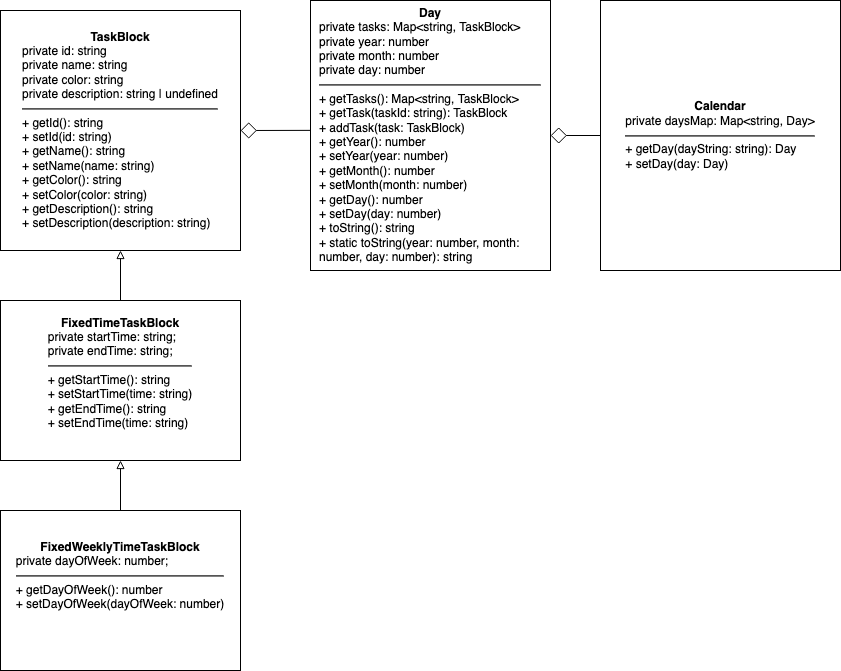
\includegraphics[width=\textwidth]{uml-diagram.png}
\end{figure}

There will be multiple types of TaskBlocks, and the \texttt{FixedTimeTaskBlock} will represent tasks that repeat daily like an Evening Routine and the \texttt{FixedWeeklyTimeTaskBlock} will represent tasks that repeat weekly like a school club meeting.

\section*{Flowchart}
\begin{figure}[H]
	\caption{A flowchart created using FigJam that represents the different actions the user can perform on my Timeblocker app.}
	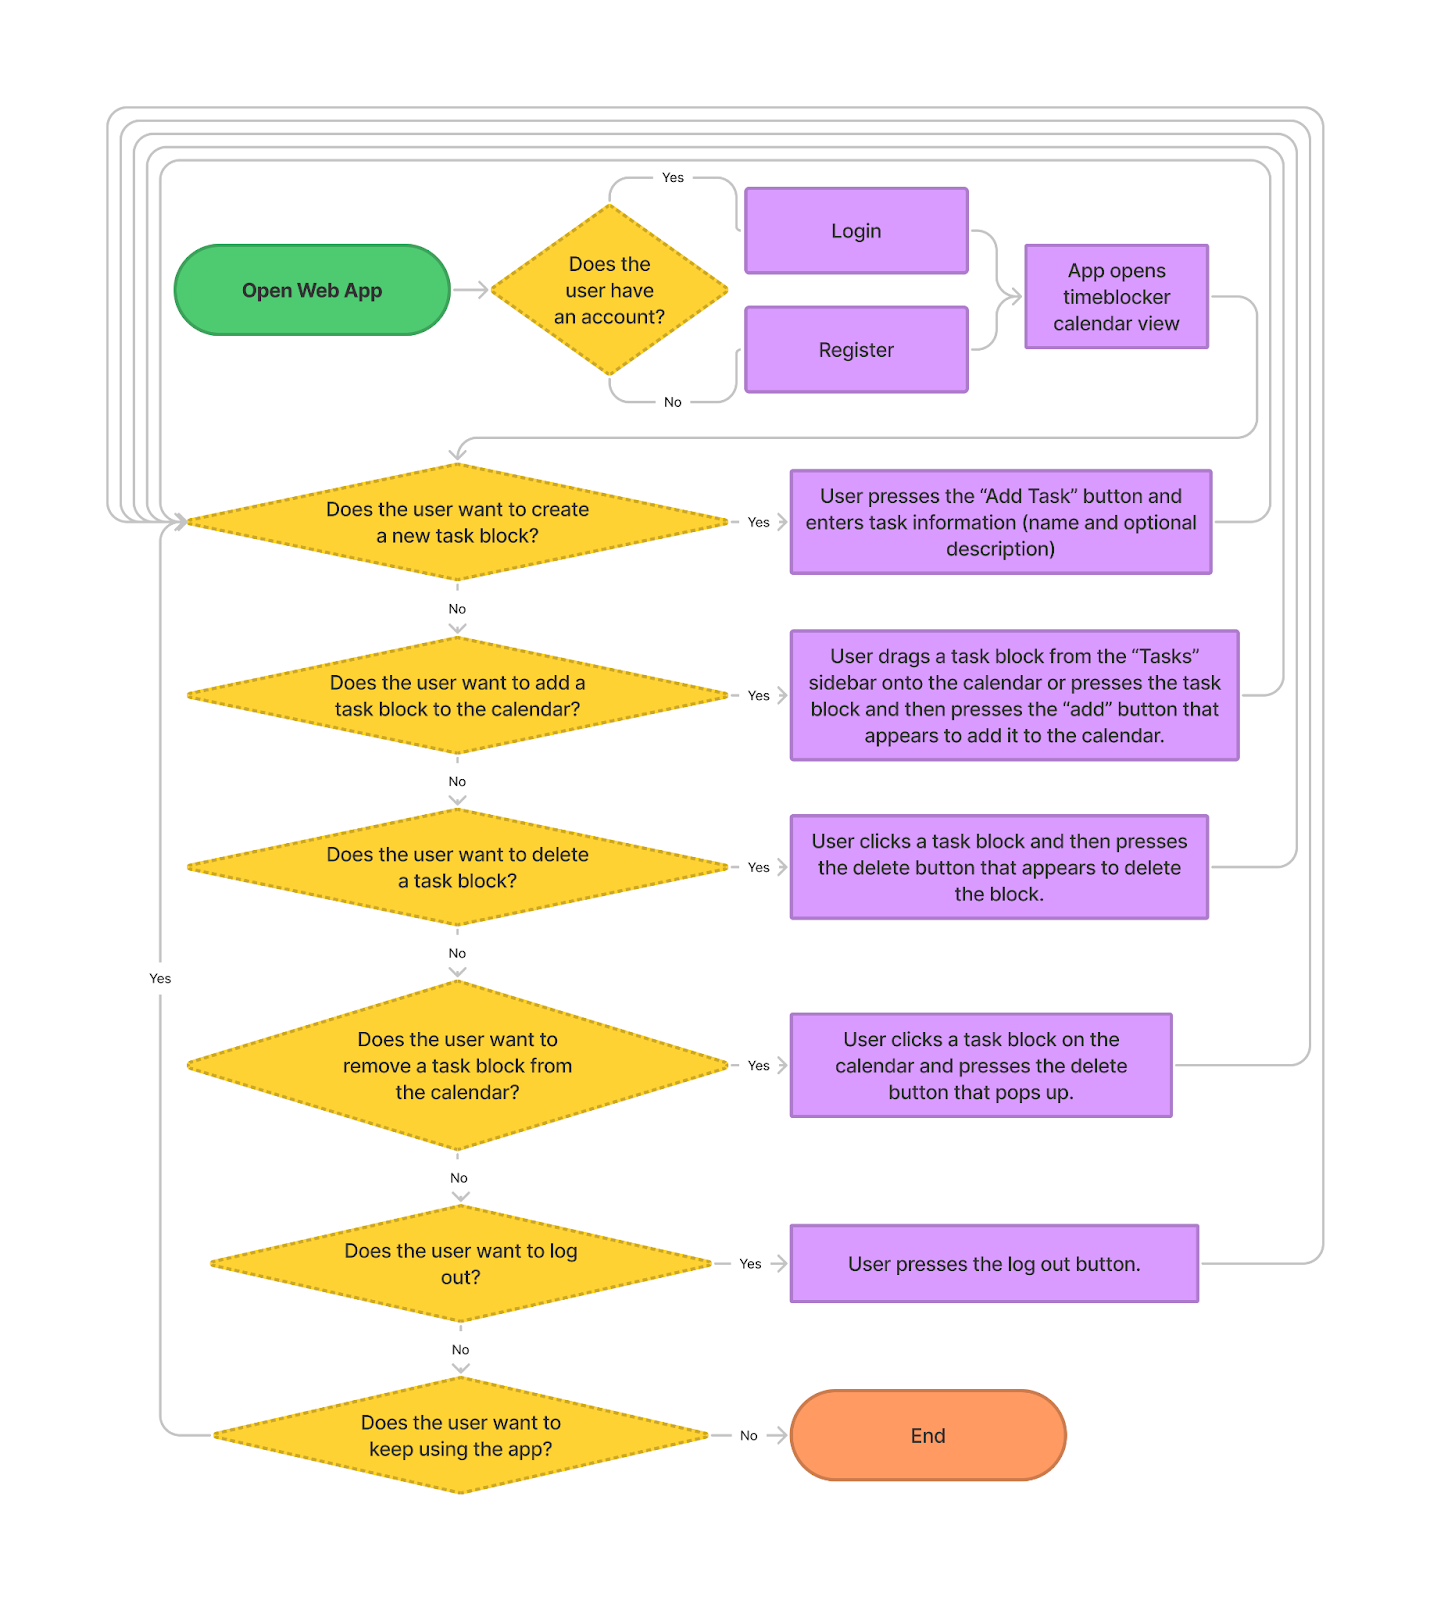
\includegraphics[width=\textwidth]{flowchart.png}
\end{figure}

\section*{UI Design}

I created the following UI designs using Figma (https://figma.com).

\subsection*{Register Page}
\begin{figure}[H]
	\caption{For the register page, the user must enter their password twice in order to make sure that they've typed it correctly.}
	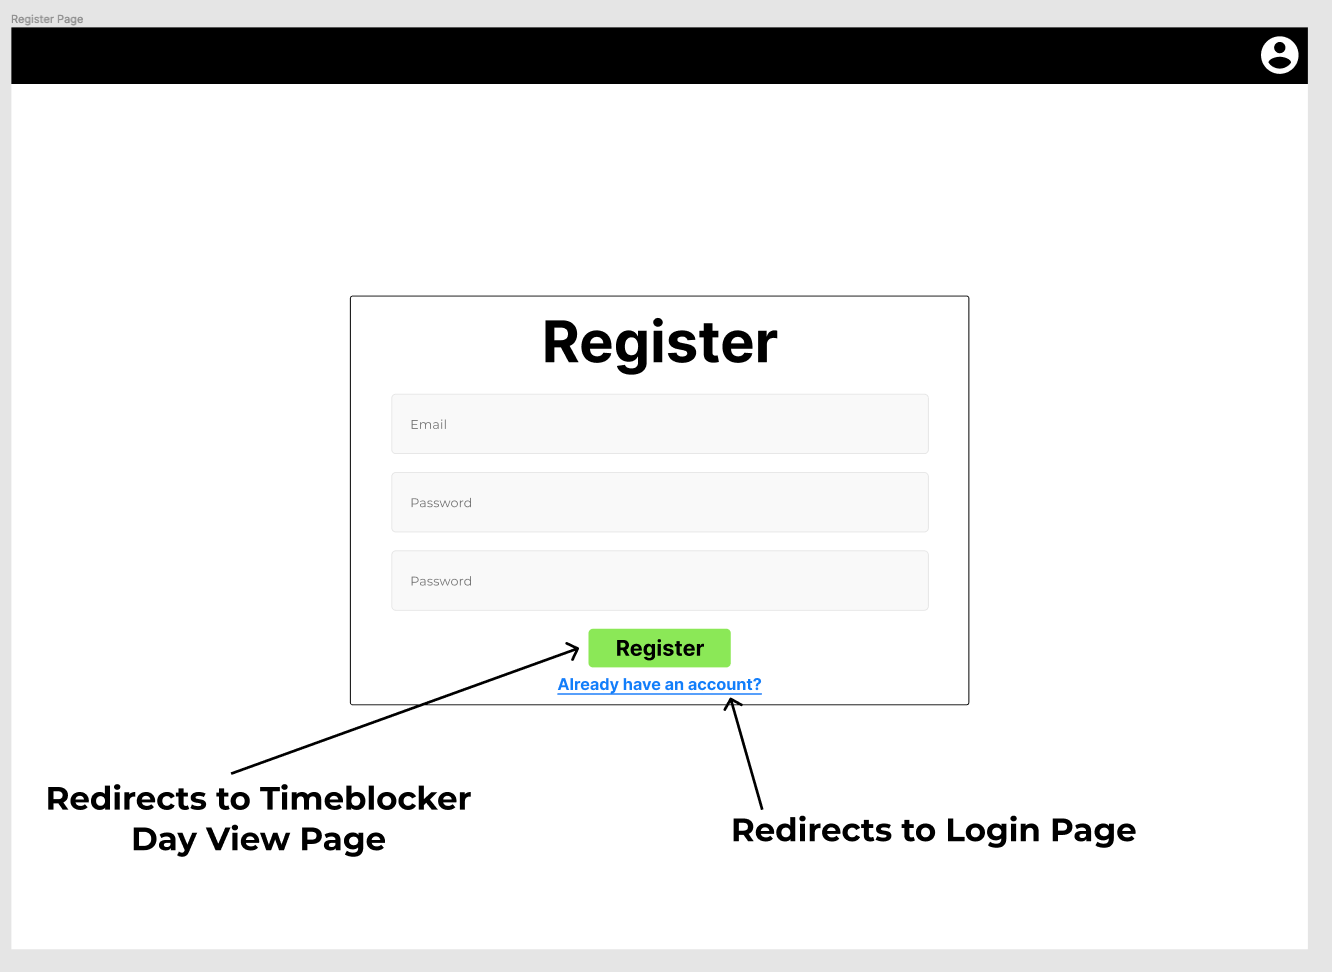
\includegraphics[width=\textwidth]{register-page.png}
\end{figure}

\subsection*{Login Page}
\begin{figure}[H]
	\caption{For the login page, the user enters the same email and password they used when registering for a new account.}
	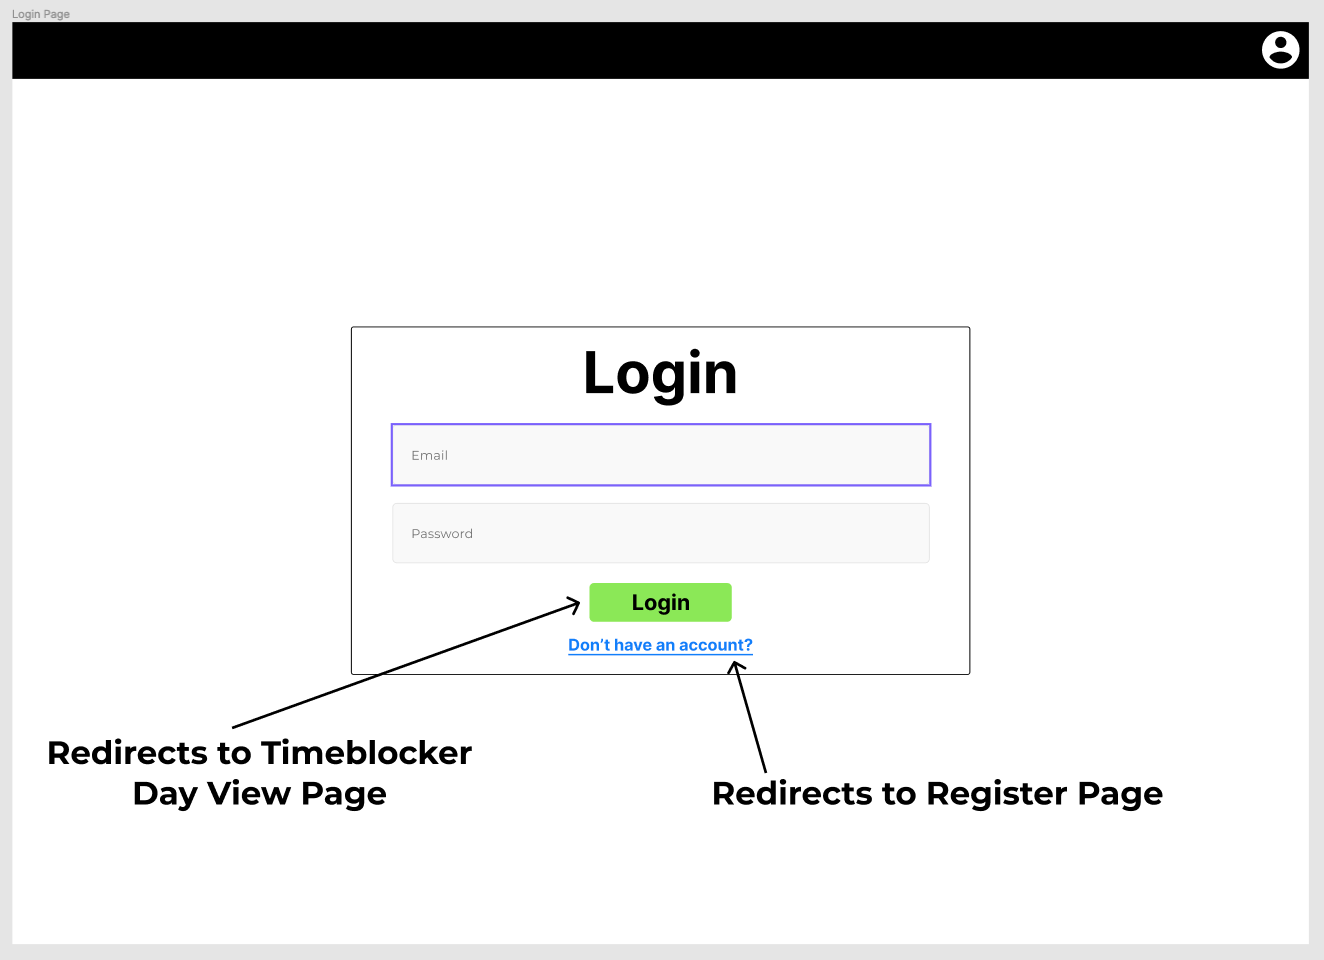
\includegraphics[width=\textwidth]{login-page.png}
\end{figure}

\subsection*{Calendar View}
\begin{figure}[H]
	\caption{The calendar view provides the user with a high level overview of their various timeblocks for each day.}
	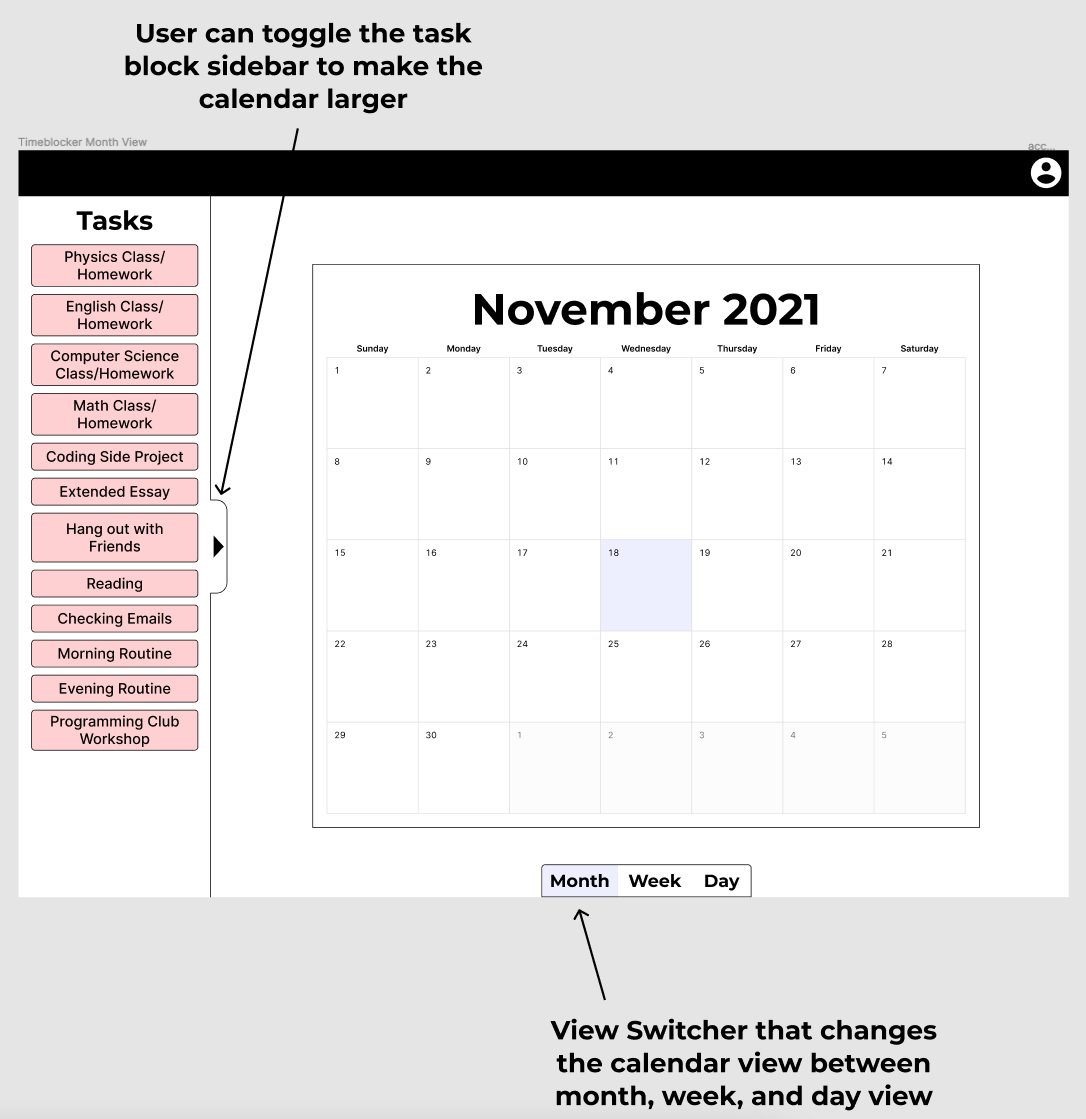
\includegraphics[width=\textwidth]{month-view.png}
\end{figure}

\subsection*{Week View}
\begin{figure}[H]
	\caption{The week view provides the user with a view of their timeblocks for the current week.}
	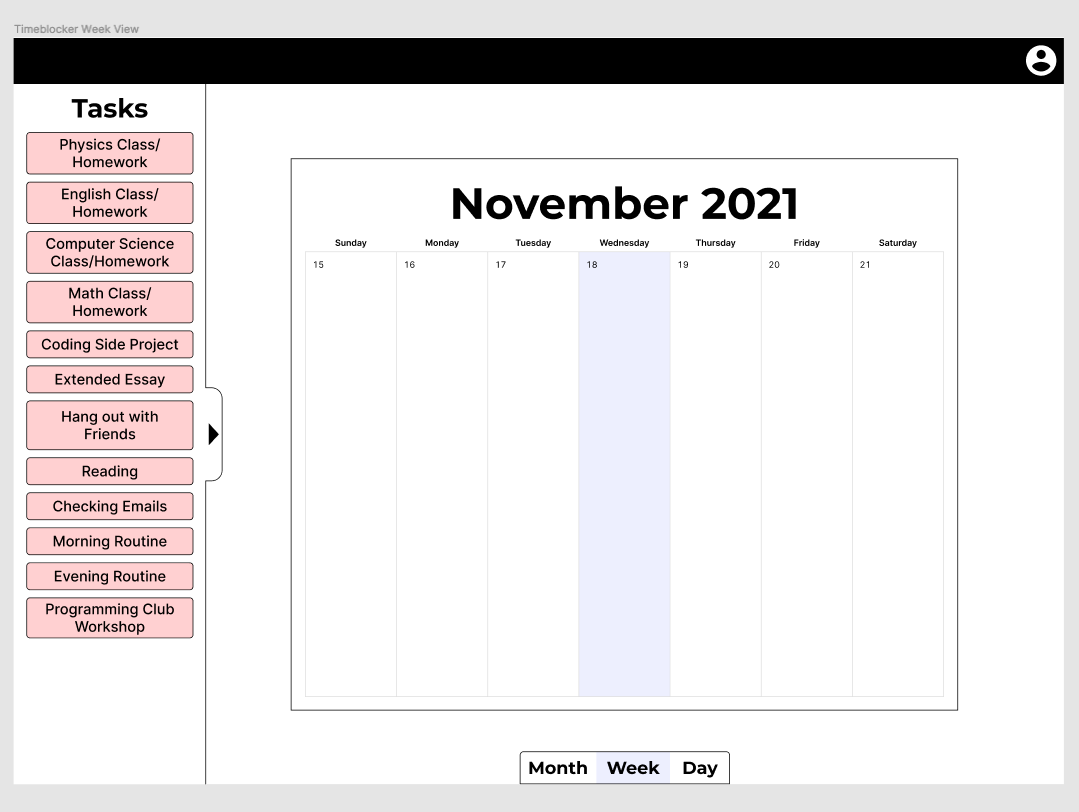
\includegraphics[width=\textwidth]{week-view.png}
\end{figure}

\subsection*{Day View}
\begin{figure}[H]
	\caption{The day view provides the user with a specific hour-by-hour breakdown of how they've scheduled their day.}
	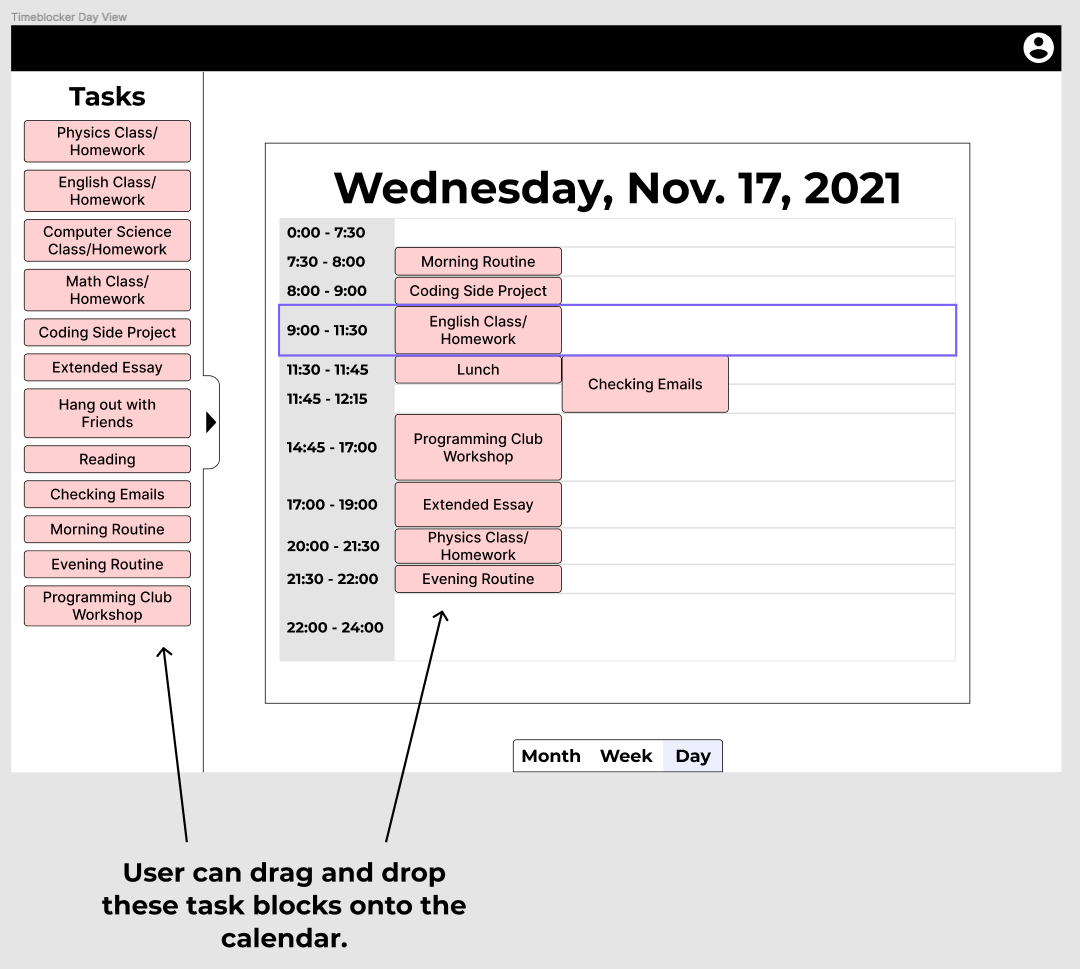
\includegraphics[width=\textwidth]{day-view.png}
\end{figure}

\newpage

\section*{Algorithms}

\subsection*{Merge Sort}

Merge sort is used to sort the tasks in alphabetical order. Because the tasks are JavaScript objects (equivalent of hashmaps in other languages), a custom comparison function must be used that compares the \texttt{name} property of the objects.

\begin{verbatim}
// The comparison function returns true if the first element is less than
// the second element
function merge (leftArray, rightArray, comparisonFunction)
  sortedArray = []
  leftIndex = 0
  rightIndex = 0

  while leftIndex < length of leftArray and rightIndex < length of rightArray
    if comparisonFunction(leftArray[leftIndex], rightArray[rightIndex])
    returns true
      add leftArray[leftIndex] to end of sortedArary
      leftIndex = leftIndex + 1
    else
      add rightArray[rightIndex] to end of sortedArray
      rightIndex = rightIndex + 1

  return sortedArray +
    remaining elements of left array +
    remaining elements of right array

function mergeSort (array, comparisonFunction)
  leftArray = first half of array
  rightArray = second half of array

  return merge(
    mergeSort(leftArray, comparisonFunction),
    mergeSort(rightArray, comparisonFunction)
  )
\end{verbatim}

\newpage

\section*{Product Development Plan}
\def\arraystretch{1.5}
\begin{xltabular}{\textwidth}{|X|X|}
	\hline
	Function
	& Comments
	\\\hline
	Landing Page
	\begin{itemize}
		\item Login/Register Button, Call to Action
		\item Features List
	\end{itemize}

	\medskip

	\textbf{Time:} 1 week
	&
	The landing page should contain a description of the app's features, as well as a call to action and the Login and Register buttons that allow the user to easily create a new account.
	\\\hline
	Account Entry Screens
	\begin{itemize}
		\item Login Screen
		\item Register Screen
	\end{itemize}
	\textbf{Time:} 3 weeks
	&
	To synchronize the user's calendar across multiple devices, they’ll need to create and log into a Timeblocker account. I need to store their information security using standard web security practices such as password hashing.
	\\\hline
	The Task Blocks Sidebar
	\begin{itemize}
		\item Ability to create, edit, and delete task blocks
		\item Sorting and searching functions.
		\item Creating different types of task blocks
	\end{itemize}
	\textbf{Time:} 3 weeks
	&
	The user needs to be able to manage their task blocks on the sidebar, with the ability to add different types of tasks and sort the tasks based on the name.
	\\\hline
	The Calendar Views
	\begin{itemize}
		\item Able to see a calendar and create a timeblock for any day on the calendar.
	\end{itemize}
	\textbf{Time:} 2 weeks
	&
	The calendar should allow the user to navigate between various months and see all the days where they've already created a timeblock. When viewing a timeblock for a specific day, the user must be able to interact with the timeblock schedule and have the ability to drag and resize tasks to reorder them.
	\\\hline
\end{xltabular}

\newpage

\section*{Testing Plan}
\begin{xltabular}{\linewidth}{|X|X|}
	\hline
	\textbf{Test Description}
	&
	\textbf{Success Criteria Fulfilled}
	\\\hline
	Creating a new account with the email ``test@example.com" with the password "password", then logging out, then trying to log back in with the same email but different password, which should give an error. Then, enter the correct password, which should log in successfully.
	&
	\vspace{-5mm}
	\begin{itemize}
		\item Registering and logging into accounts
	\end{itemize}
	\\\hline
	Creating a new task, dragging it onto the schedule, resizing the task block, renaming the task and having all timeblocks on the schedule renamed, then deleting the task and having the task on the schedule remain there (since deleting shouldn't delete tasks on the schedule in order to preserve history).
	&
	\vspace{-5mm}
	\begin{itemize}
		\item Creating, editing, and delete tasks
		\item Drag tasks onto the schedule to create task blocks
		\item Resizing the task blocks that are on the schedule
	\end{itemize}
	\\\hline
	Creating a timeblock for today and adding a task to the timeblock, then returning to the calendar, and then creating a timeblock for the following day and adding a different task to the timeblock, then returning back to the timeblock for today and seeing that the right tasks are shown on the calendar.
	&
	\vspace{-5mm}
	\begin{itemize}
		\item Creating multiple timeblocks
		\item Changing the schedule view between day and week/month
		\item Schedule autosaves every time changes are made
	\end{itemize}
	\\\hline
	Creating tasks with the names "Task 1" and "Task 2", with descriptions of "Description 3" and "Description 4" respectively, then typing in the search bar "Task 1" and only seeing the first task, and then typing in the search bar "Description 4" and only seeing the second task.
	&
	\vspace{-5mm}
	\begin{itemize}
		\item Searching through task blocks
	\end{itemize}
	\\\hline
	Opening a new browser and checking that the timeblocks are successfully saved when I log into my account. Then, create a new task on the new browser session and then closing the browser and refresh the previous browser. The new task should show up in the previous browser.
	&
	\vspace{-5mm}
	\begin{itemize}
		\item Server-side synchronization with a database to access schedules across devices
	\end{itemize}
	\\\hline
\end{xltabular}

\end{document}